\section{Pregunta N$^{\circ}$10\qquad Carlos Daniel Malvaceda Canales}

\begin{frame}
	\begin{enumerate}\setcounter{enumi}{9}
		\item

		      Determinar gráficamente el número de raíces reales de la
		      ecuación no lineal
		      \begin{math}
			      x\ln\left(x\right)=
			      1
		      \end{math}
		      y resuelve usando los métodos de la bisección, la regla
		      falsa y la regla falsa modificada para $\epsilon=10^{-5}$.
	\end{enumerate}

	\begin{solution}
            Consideramos la función  \(f(x)=xln(x)-1 \) como la función a analizar. Y según se observa graficamente esta posee una solución real.
		\begin{figure}
			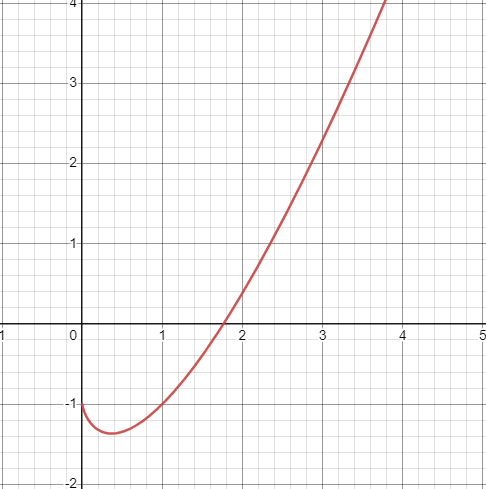
\includegraphics[width=3cm]{p10-grafica.png}
		\end{figure}
            Sin embargo también se puede determinar si posee solución real en un intervalo, según el siguiente teorema.
        \begin{figure}
			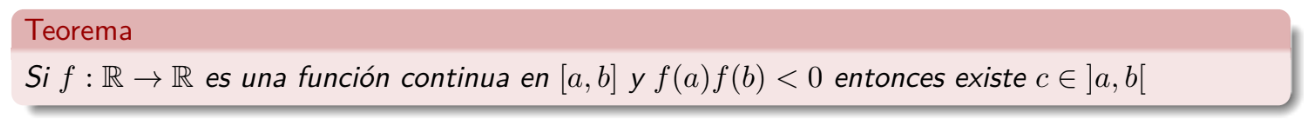
\includegraphics[width=12cm]{p10-teorema1.png}
		\end{figure}
              Por lo que si tomamos los valores para el intervalo  \(a=1,b=2\) se observa que \(f(1) f(2) < 0\), lo cual nos garantiza que en dicho intervalo existe una solución.

	\end{solution}
\end{frame}

\begin{frame}{Método de la bisección}
Previamente al calculo de la solución por el método de bisección , utilazaremos el siguiente teorema para calcular cuantas iteraciones usaremos.
        \begin{figure}
			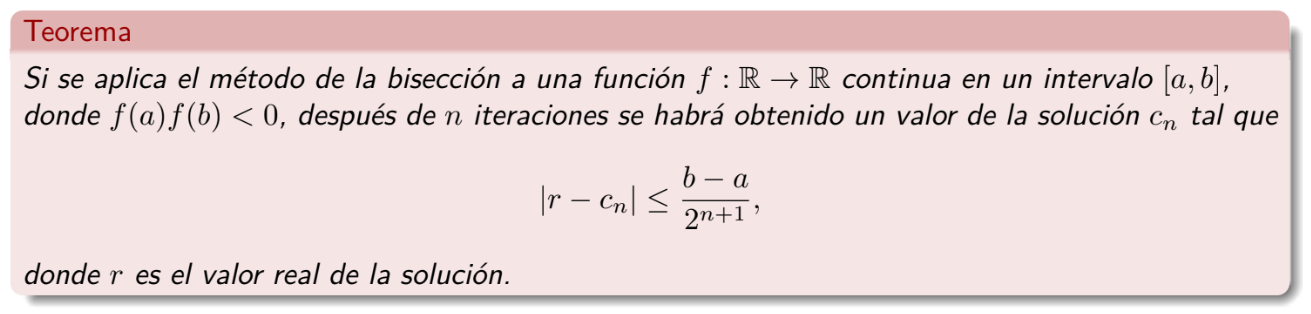
\includegraphics[width=11cm]{p10-teorema2.png}
		\end{figure}
De aquí podemos calcular \(n\) si una tolerancia para el error \( \epsilon \) , es dada por :
\begin{equation*}
    n = \ | \log_2 (\frac{b-a}{\epsilon}) \ | = \ | \log_2 (\frac{2-1}{10^{-5}}) \ | = 17
\end{equation*}

Ahora el método de la bisección consiste en encontrar un intervalo \( [a, b] \) que contiene la solución y
tomar el punto medio como una aproximación de \( x∗ \) , luego escogemos el nuevo intervalo de
búsqueda \( [a, c] \) o \( [c, b] \) considerando el cambio de signo de \( f \).
\end{frame}

\begin{frame}{Método de la bisección}
         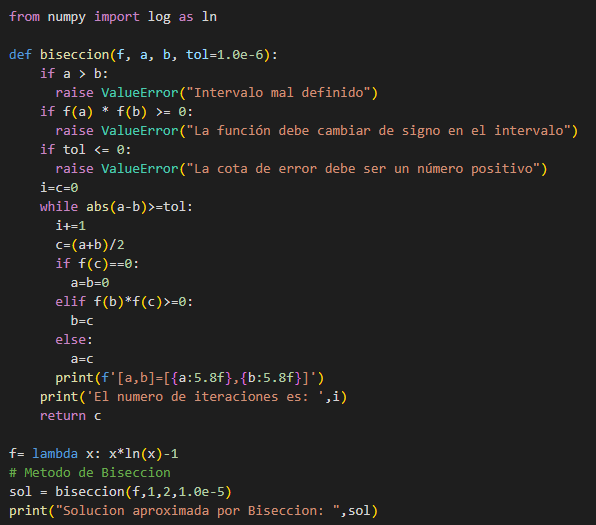
\includegraphics[width=8cm]{p10-codigo-biseccion.png}
        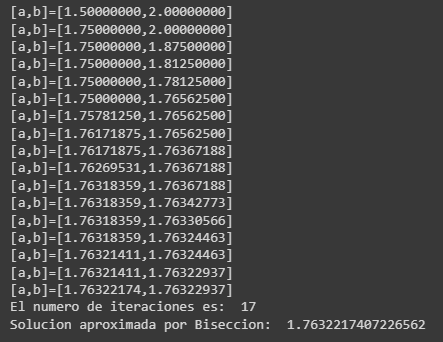
\includegraphics[width=6cm]{p10-ejecucion-biseccion.png}
\end{frame}

\begin{frame}{Regla Falsa}
    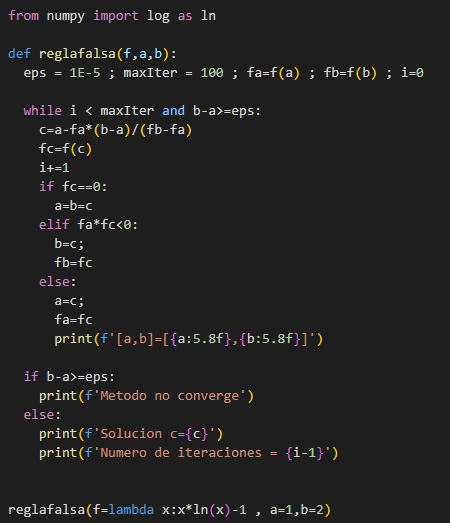
\includegraphics[width=6cm]{p10-codigo-regla-falsa.png}
        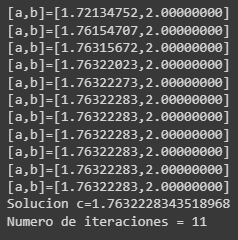
\includegraphics[width=4cm]{p10-ejecucion-regla-falsa.png}
\end{frame}
\begin{frame}{Regla Falsa Modificada}
    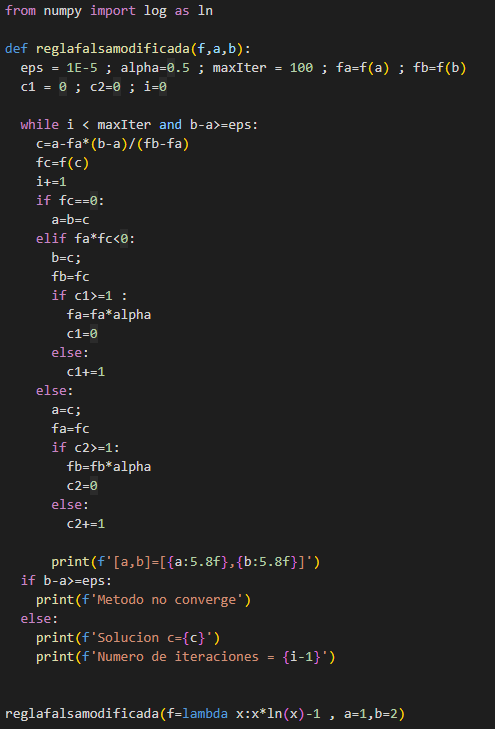
\includegraphics[width=5cm]{p10-codigo-regla-falsa-modificada.png}
        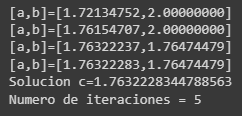
\includegraphics[width=5cm]{p10-ejecucion-regla-falsa-modificada.png}
\end{frame}
